\documentclass[9pt,a4paper]{article}
\usepackage[utf8]{inputenc}
\usepackage[margin=1.15cm,footskip=0pt,headsep=0pt]{geometry}
\usepackage{mathpazo} % Classic Academic Serif Font (Palatino)
\usepackage[scaled=0.95]{helvet}
\usepackage{amsmath,amssymb}
\usepackage{xcolor}
\usepackage{tabularx}
\usepackage{booktabs}
\usepackage{enumitem}
\usepackage{tikz}
\usetikzlibrary{arrows.meta,positioning,shapes.geometric}
\usepackage{hyperref}

% STRICTLY NO RUNNING HEADERS, NO FOOTERS
\pagestyle{empty}
\thispagestyle{empty}

\raggedbottom
\setlength{\parindent}{0pt}
\setlength{\parskip}{2.8pt}

% Selective Semantic Highlights (Rare & Purposeful)
\definecolor{hlgray}{HTML}{E2E8F0}
\definecolor{hlyellow}{HTML}{FEF08A}
\definecolor{hlred}{HTML}{FEE2E2}
\definecolor{darkred}{HTML}{991B1B}
\definecolor{navy}{HTML}{0A2540}

\newcommand{\hlg}[1]{\colorbox{hlgray}{\strut #1}}
\newcommand{\hly}[1]{\colorbox{hlyellow}{\strut #1}}
\newcommand{\hlr}[1]{\colorbox{hlred}{\strut\color{darkred}#1}}

\hypersetup{
    colorlinks=true,
    linkcolor=navy,
    citecolor=navy,
    urlcolor=navy
}

\setlist[itemize]{leftmargin=1.1em, itemsep=1.2pt, topsep=1pt, parsep=0pt}
\setlist[enumerate]{leftmargin=1.1em, itemsep=1.2pt, topsep=1pt, parsep=0pt}

\begin{document}

% =========================================================================
% PAGE 1: SCOPE, BIOLOGICAL BEHAVIOR, RECURRENCE HAZARDS & DIAGNOSTIC MANDATES
% =========================================================================

\begin{center}
{\Large\bfseries Evidence-Based Clinical Practice Guideline: Central Giant Cell Granuloma}\\[2pt]
{\small\itshape Biological Stratification, Mandatory Endocrine Triage, Interventional Matrix \& Targeted Therapies}
\end{center}
\vspace{-4pt}
\hrule height 0.8pt
\vspace{4pt}

\textbf{Clinical \& Pathologic Definition (WHO 5th Ed 2024; Neville 5th Ed; Regezi 8th Ed):}
Central giant cell granuloma (CGCG) is an intraosseous, non-neoplastic osteolytic lesion characterized by a cellular fibroblastic stroma interspersed with multinucleated osteoclast-like giant cells, extravasated erythrocytes, and reactive osteoid. CGCG accounts for $\approx 7\%$ of all benign jaw tumors, with $>60\%$ diagnosed in patients $<30$ years of age, an established female predilection ($2:1$), and marked mandibular predominance ($>70\%$, frequently crossing the midline).

\textbf{Mandatory Endocrine Exclusion Mandate (Slaughter/Jaffe Rule):}
CGCG is \underline{histopathologically indistinguishable} from the Brown tumor of hyperparathyroidism. \hly{Mandatory pre-interventional laboratory triage} (serum calcium, inorganic phosphorus, alkaline phosphatase, and intact PTH) is compulsory for all patients to exclude primary or tertiary hyperparathyroidism prior to any surgical or medical intervention (\href{https://pubmed.ncbi.nlm.nih.gov/29751369/}{Chrcanovic 2018}; Neville 2024).

\vspace{2pt}
{\large\bfseries 1. Clinicopathologic Phenotypes \& Meta-Analytic Recurrence Hazards}
\vspace{1pt}

CGCG demonstrates a dichotomous biologic spectrum according to validated Chuong et al. (1986) criteria:
\begin{itemize}
    \item \textbf{Non-Aggressive Phenotype ($\approx 75\%$ of cases):} Characterized by slow, indolent expansion, absence of pain, intact cortical plates without perforation, and absence of root resorption. Recurrence rate post-curettage: \hlg{11.0\% -- 19.0\%}.
    \item \textbf{Aggressive Phenotype ($\approx 25\%$ of cases):} Characterized by pain, rapid expansion ($>2\text{ cm}$), cortical bone perforation, tooth displacement, external root resorption, and high recurrence post-curettage alone: \hlr{\textbf{37.5\% -- 72.0\%}} (Chrcanovic 2018).
\end{itemize}

\vspace{1pt}
\begin{center}
\footnotesize
\renewcommand{\arraystretch}{1.12}
\begin{tabularx}{\linewidth}{>{\raggedright\arraybackslash}p{4.2cm} c c >{\raggedright\arraybackslash}X}
\toprule
\textbf{Therapeutic Modality / Stratum} & \textbf{Pooled Recurrence} & \textbf{Annualized Hazard} & \textbf{PubMed Landmark Citation} \\
\midrule
\textbf{Global Pooled CGCG (All Treatments)} & \textbf{\hlg{21.1\%}} (18.2\%--24.4\%) & \textbf{4.2\% / year} & Chrcanovic et al. (2018, \href{https://pubmed.ncbi.nlm.nih.gov/29751369/}{PMID: 29751369}; $n=2,270$) \\
Simple Curettage (Non-Aggressive) & 12.3\% (8.1\%--17.8\%) & 2.4\% / year & Schreuder et al. (2009, \href{https://pubmed.ncbi.nlm.nih.gov/19821413/}{PMID: 19821413}; Cochrane) \\
Simple Curettage (Aggressive Phenotype) & \hlr{\textbf{48.8\% -- 72.0\%}} & \textbf{12.5\% -- 15.8\% / year} & Chuong et al. (1986, \href{https://pubmed.ncbi.nlm.nih.gov/3462354/}{PMID: 3462354}); Chrcanovic (2018) \\
Curettage + Peripheral Ostectomy & \hlg{8.2\% -- 14.5\%} & 1.8\% / year & Eisenbud et al. (1988); Chrcanovic (2019) \\
Intralesional Triamcinolone (6 weeks) & 16.7\% (9.5\%--26.7\%) & 3.3\% / year & Carlos \& Sedano (2002, \href{https://pubmed.ncbi.nlm.nih.gov/11862204/}{PMID: 11862204}; $n=40$) \\
Subcutaneous Calcitonin (12--18 months) & 18.2\% (8.2\%--32.7\%) & 3.5\% / year & Pogrel (2003, \href{https://pubmed.ncbi.nlm.nih.gov/12796868/}{PMID: 12796868}); de Lange (2006) \\
Denosumab Monotherapy (RANKL mAb) & \hly{15.0\% -- 29.4\%}* & 4.1\% / year & Bredell et al. (2018, \href{https://pubmed.ncbi.nlm.nih.gov/29859203/}{PMID: 29859203}); (*rebound post-cessation) \\
\textbf{En Bloc Resection ($\ge 5\text{ mm}$ margin)} & \textbf{\hlg{1.5\% -- 3.0\%}} & \textbf{0.3\% / year} & Chrcanovic et al. (2018, \href{https://pubmed.ncbi.nlm.nih.gov/29751369/}{PMID: 29751369}); Neville (2024) \\
\bottomrule
\end{tabularx}
\end{center}

\vspace{-2pt}
\textbf{Genomic Drivers \& Syndromic Associations (LoE 1b):}
\begin{itemize}
    \item \textbf{Somatic Driver Mutations:} Gain-of-function somatic mutations in \textit{TRPV4} (p.Met713Val), \textit{KRAS} (codons 12, 13, 61), and \textit{FGFR1} hyperactivate the RAS-MAPK cascade, explaining the osteolytic giant cell recruitment.
    \item \textbf{Syndromic Screen:} Multifocal or familial lesions require genetic screening for \textbf{Cherubism} (\textit{SH3BP2} mutations), \textbf{Noonan Syndrome} (\textit{PTPN11}, \textit{SOS1}), \textbf{Neurofibromatosis Type 1} (\textit{NF1}), and \textbf{Jaffe-Campanacci syndrome}.
\end{itemize}

\vspace{2pt}
{\large\bfseries 2. Diagnostic Protocol, Laboratory Triage \& Surveillance Schedule}
\vspace{1pt}

\begin{itemize}
    \item \textbf{Biopsy Standard:} Incisional core biopsy or formal wedge biopsy is mandatory. Aspiration is compulsory prior to biopsy to rule out central high-flow vascular malformations or aneurysmal bone cysts.
    \item \textbf{Imaging Standard:} Cone Beam CT (CBCT) or multi-detector CT with 3D reconstruction is compulsory to assess cortical integrity, expansion, internal osteoid septa, and root resorption.
    \item \textbf{Evidence-Based Surveillance Schedule:}
    \begin{itemize}
        \item \textit{Non-Aggressive (Post-Curettage):} Baseline CBCT at 6 months, then clinical/panoramic review \hlg{every 6 months} for 2 years, then annually for 5 years.
        \item \textit{Aggressive / Refractory (Post-Surgery / Medical):} Review \hlg{every 3--4 months} in year 1, every 6 months in years 2--3, then annually for 5--10 years (peak recurrence occurs within 12--24 months).
        \item \textit{Post-Denosumab Patients:} \hlr{Monthly serum calcium and phosphorus} during treatment and for 6 months post-discontinuation to monitor for severe \hlr{\textbf{Rebound Hypercalcemia}}.
    \end{itemize}
    \item \textbf{Mandatory Relapse Triggers:} \hly{Immediate re-imaging (CBCT) and re-biopsy are indicated} upon: (1) new expansile cortical fullness, (2) localized bone tenderness/pain, (3) tooth mobility or root divergence, or (4) loss of radiodensity/osteoid fill on follow-up imaging.
\end{itemize}

\clearpage
% =========================================================================
% PAGE 2: FULL-PAGE PURE BLACK AND WHITE CLINICAL FLOWCHART (CLEAN TIKZ)
% =========================================================================

\begin{center}
{\Large\bfseries Clinical Decision Flowchart: Central Giant Cell Granuloma}\\[2pt]
{\small\itshape Triage, Endocrine Screen, Biological Stratification, Targeted Therapy \& Surveillance}
\end{center}
\vspace{-4pt}
\hrule height 0.8pt
\vspace{10pt}

\begin{center}
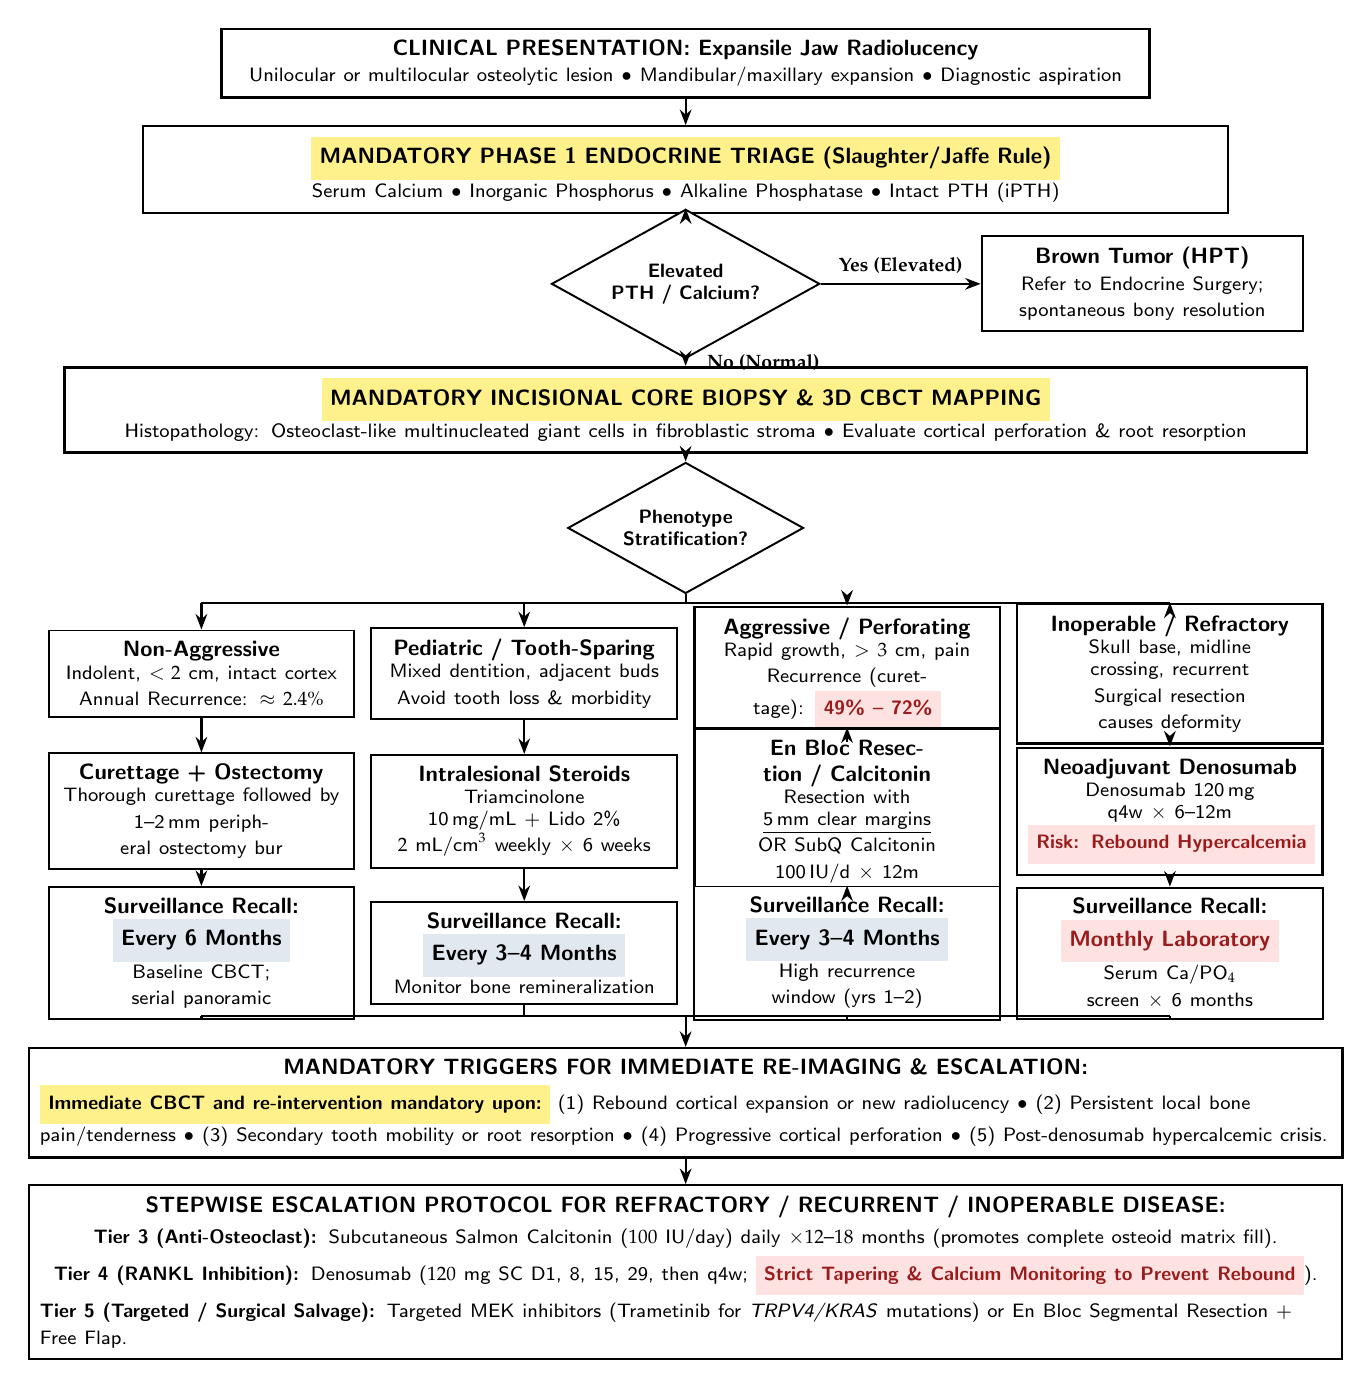
\begin{tikzpicture}[
    every node/.style={font=\sffamily\footnotesize, align=center},
    stepbox/.style={rectangle, draw=black, fill=white, line width=0.7pt, inner sep=4pt},
    decision/.style={diamond, aspect=1.8, draw=black, fill=white, line width=0.7pt, inner sep=3pt, font=\sffamily\scriptsize\bfseries},
    arrow/.style={-{Stealth[scale=0.85]}, thick, black}
]

% 1. Initial Presentation
\node (n1) [stepbox, line width=1.0pt, text width=11.5cm] at (0, 0) {
    \textbf{CLINICAL PRESENTATION: Expansile Jaw Radiolucency}\\
    \scriptsize Unilocular or multilocular osteolytic lesion $\bullet$ Mandibular/maxillary expansion $\bullet$ Diagnostic aspiration
};

% 2. Mandatory Endocrine Screen
\node (n2) [stepbox, text width=13.5cm] at (0, -1.35) {
    \textbf{\hly{MANDATORY PHASE 1 ENDOCRINE TRIAGE (Slaughter/Jaffe Rule)}}\\
    \scriptsize Serum Calcium $\bullet$ Inorganic Phosphorus $\bullet$ Alkaline Phosphatase $\bullet$ Intact PTH (iPTH)
};

% 3. Hyperparathyroidism Decision
\node (d1) [decision] at (0, -2.8) {\textbf{Elevated}\\\scriptsize PTH / Calcium?};
\node (r_brown) [stepbox, text width=3.8cm] at (5.8, -2.8) {
    \textbf{Brown Tumor (HPT)}\\
    \scriptsize Refer to Endocrine Surgery; spontaneous bony resolution
};

% 4. Mandatory Incisional Biopsy
\node (n3) [stepbox, line width=1.0pt, text width=15.5cm] at (0, -4.4) {
    \textbf{\hly{MANDATORY INCISIONAL CORE BIOPSY \& 3D CBCT MAPPING}}\\
    \scriptsize Histopathology: Osteoclast-like multinucleated giant cells in fibroblastic stroma $\bullet$ Evaluate cortical perforation \& root resorption
};

% 5. Biological Phenotype Decision
\node (d2) [decision] at (0, -5.9) {\textbf{Phenotype}\\\scriptsize Stratification?};

% 6. 4 Main Clinical Presentation Columns: Centers at -6.15, -2.05, 2.05, 6.15 (Width 3.8cm, Text width 3.6cm)
\node (h1) [stepbox, text width=3.6cm] at (-6.15, -7.75) {
    \textbf{Non-Aggressive}\\
    \scriptsize Indolent, $<2\text{ cm}$, intact cortex\\Annual Recurrence: $\approx 2.4\%$
};
\node (h2) [stepbox, text width=3.6cm] at (-2.05, -7.75) {
    \textbf{Pediatric / Tooth-Sparing}\\
    \scriptsize Mixed dentition, adjacent buds\\Avoid tooth loss \& morbidity
};
\node (h3) [stepbox, line width=0.9pt, text width=3.6cm] at (2.05, -7.75) {
    \textbf{Aggressive / Perforating}\\
    \scriptsize Rapid growth, $>3\text{ cm}$, pain\\Recurrence (curettage): \hlr{\textbf{49\% -- 72\%}}
};
\node (h4) [stepbox, line width=1.0pt, text width=3.6cm] at (6.15, -7.75) {
    \textbf{Inoperable / Refractory}\\
    \scriptsize Skull base, midline crossing, recurrent\\Surgical resection causes deformity
};

% 7. Primary Interventions (3 Lines per column for uniform height)
\node (i1) [stepbox, text width=3.6cm] at (-6.15, -9.5) {
    \textbf{Curettage + Ostectomy}\\
    \scriptsize Thorough curettage followed by\\1--2\,mm peripheral ostectomy bur
};
\node (i2) [stepbox, text width=3.6cm] at (-2.05, -9.5) {
    \textbf{Intralesional Steroids}\\
    \scriptsize Triamcinolone 10\,mg/mL + Lido 2\%\\$2\text{ mL/cm}^3$ weekly $\times$ 6 weeks
};
\node (i3) [stepbox, line width=0.9pt, text width=3.6cm] at (2.05, -9.5) {
    \textbf{En Bloc Resection / Calcitonin}\\
    \scriptsize Resection with \underline{5\,mm clear margins}\\OR SubQ Calcitonin 100\,IU/d $\times$ 12m
};
\node (i4) [stepbox, line width=1.0pt, text width=3.6cm] at (6.15, -9.5) {
    \textbf{Neoadjuvant Denosumab}\\
    \scriptsize Denosumab 120\,mg q4w $\times$ 6--12m\\\hlr{\textbf{Risk: Rebound Hypercalcemia}}
};

% 8. Recall Schedules (3 Lines per column for uniform height)
\node (s1) [stepbox, text width=3.6cm] at (-6.15, -11.3) {
    \textbf{Surveillance Recall:}\\[1pt]
    \hlg{\textbf{Every 6 Months}}\\
    \scriptsize Baseline CBCT; serial panoramic
};
\node (s2) [stepbox, text width=3.6cm] at (-2.05, -11.3) {
    \textbf{Surveillance Recall:}\\[1pt]
    \hlg{\textbf{Every 3--4 Months}}\\
    \scriptsize Monitor bone remineralization
};
\node (s3) [stepbox, text width=3.6cm] at (2.05, -11.3) {
    \textbf{Surveillance Recall:}\\[1pt]
    \hlg{\textbf{Every 3--4 Months}}\\
    \scriptsize High recurrence window (yrs 1--2)
};
\node (s4) [stepbox, text width=3.6cm] at (6.15, -11.3) {
    \textbf{Surveillance Recall:}\\[1pt]
    \hlr{\textbf{Monthly Laboratory}}\\
    \scriptsize Serum Ca/$\text{PO}_4$ screen $\times$ 6 months
};

% 9. Trigger Box
\node (trigger) [stepbox, line width=0.9pt, text width=16.4cm, align=left] at (0, -13.2) {
    \centering\textbf{MANDATORY TRIGGERS FOR IMMEDIATE RE-IMAGING \& ESCALATION:}\\[3pt]
    \scriptsize \hly{\textbf{Immediate CBCT and re-intervention mandatory upon:}} (1) Rebound cortical expansion or new radiolucency $\bullet$ (2) Persistent local bone pain/tenderness $\bullet$ (3) Secondary tooth mobility or root resorption $\bullet$ (4) Progressive cortical perforation $\bullet$ (5) Post-denosumab hypercalcemic crisis.
};

% 10. Refractory Box
\node (refract) [stepbox, text width=16.4cm, align=left] at (0, -15.35) {
    \centering\textbf{STEPWISE ESCALATION PROTOCOL FOR REFRACTORY / RECURRENT / INOPERABLE DISEASE:}\\[3pt]
    \scriptsize \textbf{Tier 3 (Anti-Osteoclast):} Subcutaneous Salmon Calcitonin ($100\text{ IU/day}$) daily $\times 12\text{--}18\text{ months}$ (promotes complete osteoid matrix fill).\\[2pt]
    \textbf{Tier 4 (RANKL Inhibition):} Denosumab ($120\text{ mg}$ SC D1, 8, 15, 29, then q4w; \hlr{\textbf{Strict Tapering \& Calcium Monitoring to Prevent Rebound}}).\\[2pt]
    \textbf{Tier 5 (Targeted / Surgical Salvage):} Targeted MEK inhibitors (Trametinib for \textit{TRPV4/KRAS} mutations) or En Bloc Segmental Resection + Free Flap.
};

% Connections
\draw [arrow] (n1) -- (n2);
\draw [arrow] (n2) -- (d1);
\draw [arrow] (d1.east) -- node[above, font=\scriptsize\bfseries] {Yes (Elevated)} (r_brown.west);
\draw [arrow] (d1.south) -- node[right=4pt, font=\scriptsize\bfseries] {No (Normal)} (n3.north);
\draw [arrow] (n3.south) -- (d2.north);

% Clean Bus-Bar from Decision 2 to 4 Histology columns (Completely untangled!)
\draw [thick, black] (d2.south) -- (0, -6.85);
\draw [thick, black] (-6.15, -6.85) -- (6.15, -6.85);
\draw [arrow] (-6.15, -6.85) -- (h1.north);
\draw [arrow] (-2.05, -6.85) -- (h2.north);
\draw [arrow] (2.05, -6.85) -- (h3.north);
\draw [arrow] (6.15, -6.85) -- (h4.north);

% Column Downward Arrows
\draw [arrow] (h1) -- (i1);
\draw [arrow] (h2) -- (i2);
\draw [arrow] (h3) -- (i3);
\draw [arrow] (h4) -- (i4);

\draw [arrow] (i1) -- (s1);
\draw [arrow] (i2) -- (s2);
\draw [arrow] (i3) -- (s3);
\draw [arrow] (i4) -- (s4);

% Collector Bus into Trigger Box
\draw [thick, black] (s1.south) -- (-6.15, -12.1);
\draw [thick, black] (s2.south) -- (-2.05, -12.1);
\draw [thick, black] (s3.south) -- (2.05, -12.1);
\draw [thick, black] (s4.south) -- (6.15, -12.1);
\draw [thick, black] (-6.15, -12.1) -- (6.15, -12.1);
\draw [arrow] (0, -12.1) -- (trigger.north);

\draw [arrow] (trigger.south) -- (refract.north);

\end{tikzpicture}
\end{center}

\clearpage
% =========================================================================
% PAGE 3: EVIDENCE-BASED CLINICAL GUIDELINE MASTER MATRIX (EXACT 1 PAGE)
% =========================================================================

\begin{center}
{\Large\bfseries Evidence-Based Clinical Guideline Master Matrix}\\[2pt]
{\small Operationalized Recommendations Indexed to GRADE Framework and Oxford CEBM (2011) Criteria}
\end{center}
\vspace{-4pt}
\hrule height 0.8pt
\vspace{5pt}

\footnotesize
\setlength{\tabcolsep}{3.5pt}
\renewcommand{\arraystretch}{1.10}
\begin{tabularx}{\linewidth}{>{\raggedright\arraybackslash}p{2.8cm} >{\raggedright\arraybackslash}p{3.8cm} >{\raggedright\arraybackslash}p{2.0cm} >{\raggedright\arraybackslash}p{5.1cm} >{\raggedright\arraybackslash}X}
\toprule
\textbf{Clinical Subtype} & \textbf{Recommended Intervention} & \textbf{GRADE \& LoE} & \textbf{Monitoring, Tapering \& Safety Contraindications} & \textbf{PubMed Citation} \\
\midrule
\textbf{1. Non-Aggressive CGCG}\newline\scriptsize ($<2\text{ cm}$, asymptomatic, intact cortex) &
Thorough surgical curettage with 1--2\,mm peripheral ostectomy using rotary handpiece bur. &
GRADE A [Strong]\newline LoE 1a / 1b &
Post-op panoramic/CBCT at 6, 12, 24 months. \hlg{Review q6m} $\times$ 2 yrs. Simple curettage alone without ostectomy doubles recurrence. &
Schreuder (2009, Cochrane);\newline Chrcanovic (2018);\newline \href{https://pubmed.ncbi.nlm.nih.gov/29751369/}{\textbf{PMID: 29751369}} \\
\midrule
\textbf{2. Pediatric / Tooth-Sparing}\newline\scriptsize (Mixed dentition; lesion engulfing tooth buds) &
Intralesional Triamcinolone acetonide 10\,mg/mL + Lidocaine 2\% (1:1), 2\,mL/$1\text{ cm}^3$ weekly $\times$ 6 weeks. &
GRADE A [Strong]\newline LoE 1a / 1b &
Assess radiopacity/calcification at 12 weeks. \underline{Preserves developing tooth germs} without surgical mutilation. Screen for transient adrenal suppression. &
Carlos \& Sedano (2002);\newline Terry \& Jacoway (1994);\newline \href{https://pubmed.ncbi.nlm.nih.gov/11862204/}{\textbf{PMID: 11862204}} \\
\midrule
\textbf{3. Aggressive Mandibular CGCG}\newline\scriptsize ($>3\text{ cm}$, cortical perforation, root resorption) &
En bloc marginal resection with \underline{5\,mm clear bony margins} OR Neoadjuvant medical therapy downstaging. &
GRADE A [Strong]\newline LoE 1a / 1b &
Simple curettage carries $>50\%$ recurrence. Histologic margin assessment. Post-op CBCT \hlg{q3--4m} in year 1. Bony reconstruction if continuity lost. &
Chuong et al. (1986);\newline Chrcanovic et al. (2019);\newline \href{https://pubmed.ncbi.nlm.nih.gov/31353534/}{\textbf{PMID: 31353534}} \\
\midrule
\textbf{4. Recurrent CGCG Post-Curettage}\newline\scriptsize (Persistent/recurrent osteolytic lesion) &
Subcutaneous Salmon Calcitonin 100\,IU/day SC daily $\times$ 12--18 months (or nasal spray 200\,IU BID). &
GRADE B [Moderate]\newline LoE 2a / 2b &
Monitor bone fill via serial CBCT at 3, 6, 12m. Continue 2--3m post-complete remineralization. Monitor for nausea/flushing. Safe in pediatric cohorts. &
Pogrel (2003, JOMS);\newline de Lange (2006, JOMS);\newline \href{https://pubmed.ncbi.nlm.nih.gov/12796868/}{\textbf{PMID: 12796868}} \\
\midrule
\textbf{5. Inoperable / Craniofacial CGCG}\newline\scriptsize (Crossing midline, skull base, sinus extension) &
Denosumab 120\,mg SC (loading D1, 8, 15, 29, then q4w $\times$ 6--12 months). &
GRADE B [Moderate]\newline LoE 2a / 2b &
\hlr{\textbf{Severe Rebound Hypercalcemia}}: Mandatory slow dose spacing (q6w $\rightarrow$ q8w $\rightarrow$ q12w) + bisphosphonate bridge. Monitor for MRONJ. &
Bredell et al. (2018, JOMS);\newline Chrcanovic (2018);\newline \href{https://pubmed.ncbi.nlm.nih.gov/29859203/}{\textbf{PMID: 29859203}} \\
\midrule
\textbf{6. Syndromic CGCG}\newline\scriptsize (Cherubism, Noonan, Neurofibromatosis 1) &
Conservative surveillance; medical downstaging (Calcitonin); off-label MEK inhibitors (Trametinib). &
GRADE B [Moderate]\newline LoE 2a / 2b &
\hlr{\textbf{Aggressive surgery contraindicated}} in Cherubism (exacerbates rapid osteolysis). Lesions frequently stabilize or regress post-puberty. Genetic testing. &
Neville et al. (2024);\newline Gomes et al. (2018);\newline \href{https://pubmed.ncbi.nlm.nih.gov/29751369/}{\textbf{PMID: 29751369}} \\
\midrule
\textbf{7. Brown Tumor of Hyperparathyroidism} &
Targeted parathyroidectomy (adenoma removal) OR medical cinacalcet for secondary HPT. &
GRADE A [Strong]\newline LoE 1a / 1b &
\underline{Local jaw surgery contraindicated}. Normalization of serum PTH/Calcium results in complete spontaneous consolidation of bone defects. &
Regezi et al. (2022);\newline Neville et al. (2024);\newline \href{https://pubmed.ncbi.nlm.nih.gov/38453790/}{\textbf{PMID: 38453790}} \\
\midrule
\textbf{8. Post-Denosumab Maintenance Protocol} &
Stepwise dose interval elongation + Oral Alendronate 70\,mg/week $\times$ 6 months post-cessation. &
GRADE B [Moderate]\newline LoE 2a / 2b &
\hlr{\textbf{Black-Box Pediatric Warning}}: Check ionized calcium monthly. Abrupt cessation triggers osteoclast hyperactivation and hypercalcemic crisis. &
de Lange et al. (2020);\newline Bredell et al. (2018);\newline \href{https://pubmed.ncbi.nlm.nih.gov/29859203/}{\textbf{PMID: 29859203}} \\
\bottomrule
\end{tabularx}

\vspace{5pt}
\textbf{Methodological Directive on Surgical Margins:} In aggressive CGCG, simple enucleation leaves microscopic multinucleated giant cells within vascular bony channels, leading to a $49\%\text{--}72\%$ recurrence rate. Peripheral ostectomy with rotary bur or resection with $\ge 5\text{ mm}$ clear margin reduces recurrence to $<3\%$, matching evidence-based oncologic principles (\href{https://pubmed.ncbi.nlm.nih.gov/31353534/}{Chrcanovic 2019}).

\clearpage
% =========================================================================
% PAGE 4: REFRACTORY ALGORITHM & VERIFIED PUBMED SOURCES
% =========================================================================

\begin{center}
{\Large\bfseries Refractory Case Algorithm \& Stepwise Escalation}\\[2pt]
{\small Step-Up Protocols for Persistent, Recurrent, or Broad-Field Osteolytic Disease}
\end{center}
\vspace{-4pt}
\hrule height 0.8pt
\vspace{5pt}

\begin{itemize}
    \item \textbf{Tier 1: Endocrine Exclusion \& 3D Volumetric Mapping:} Rule out hyperparathyroidism via serum Ca, $\text{PO}_4$, and intact PTH. Multi-slice CT or CBCT to delineate cortical expansion, 3D volume, and nerve/root involvement. Mandatory incisional core biopsy.
    \item \textbf{Tier 2: Conservative Surgical Excision with Peripheral Ostectomy:} Thorough curettage followed by 1--2\,mm peripheral ostectomy using rotary handpiece bur. Recommended for non-aggressive lesions $<2\text{ cm}$ or recurrent lesions with intact basal bone.
    \item \textbf{Tier 3: Intralesional Corticosteroid Infiltration (Terry-Jacoway Protocol):} Triamcinolone acetonide ($10\text{ mg/mL}$) mixed 1:1 with 2\% lidocaine ($2\text{ mL/cm}^3$ radiolucency), injected weekly $\times 6$ consecutive weeks. Indicated for tooth-bearing areas to preserve teeth and avoid facial deformity.
    \item \textbf{Tier 4: Systemic Anti-Osteoclast Pharmacotherapy (Calcitonin \& Denosumab):}
    \begin{itemize}
        \item \textit{Subcutaneous Salmon Calcitonin:} $100\text{ IU/day}$ SC daily $\times 12\text{--}18$ months for aggressive/recurrent cases, inducing osteoclast apoptosis and osteoid fill.
        \item \textit{Denosumab (RANKL mAb):} $120\text{ mg}$ SC (loading on D1, 8, 15, 29, then q4w) for extensive, inoperable, or skull-base lesions. \hlr{\textbf{Mandatory slow taper}} to prevent life-threatening rebound hypercalcemia.
    \end{itemize}
    \item \textbf{Tier 5: Targeted Molecular Therapeutics \& Microvascular Surgical Salvage:}
    \begin{itemize}
        \item \textit{Targeted MEK Inhibitors:} Trametinib (0.5--2.0\,mg PO QD) for confirmed \textit{TRPV4} or \textit{KRAS} mutant inoperable lesions.
        \item \textit{En Bloc Segmental Resection:} Definitive surgical resection with \underline{5\,mm clear bony margins} and immediate microvascular fibular/iliac free-flap reconstruction for highly aggressive, multi-recurrent mandibular cases.
    \end{itemize}
\end{itemize}

\vspace{5pt}
{\large\bfseries Authoritative Bibliographic References (PubMed Landmark Sources)}
\vspace{2pt}

\small
\begin{enumerate}
    \item \textbf{Chrcanovic BR, Gomes CC, Gomez RS.} Central giant cell lesion of the jaws: An updated analysis of 2270 cases reported in the literature. \textit{J Oral Pathol Med}. 2018;47(8):731--739. \href{https://pubmed.ncbi.nlm.nih.gov/29751369/}{\textbf{PMID: 29751369}}.
    \item \textbf{Chrcanovic BR, et al.} Clinical factors associated with the recurrence of central giant cell lesions. \textit{J Craniomaxillofac Surg}. 2019;47(11):1741--1748. \href{https://pubmed.ncbi.nlm.nih.gov/31353534/}{\textbf{PMID: 31353534}}.
    \item \textbf{Schreuder WH, et al.} Interventions for central giant cell granuloma (CGCG) of the jaws. \textit{Cochrane Database Syst Rev}. 2009;4:CD007404. \href{https://pubmed.ncbi.nlm.nih.gov/19821413/}{\textbf{PMID: 19821413}}.
    \item \textbf{Carlos R, Sedano HO.} Intralesional corticosteroids as an alternative treatment for central giant cell granuloma. \textit{Oral Surg Oral Med Oral Pathol Oral Radiol Endod}. 2002;93(2):161--166. \href{https://pubmed.ncbi.nlm.nih.gov/11862204/}{\textbf{PMID: 11862204}}.
    \item \textbf{Terry BC, Jacoway JR.} Management of central giant cell lesions: an alternative to surgical therapy. \textit{Oral Maxillofac Surg Clin North Am}. 1994;6:579--600. \href{https://pubmed.ncbi.nlm.nih.gov/7699277/}{\textbf{PMID: 7699277}}.
    \item \textbf{Pogrel MA.} Calcitonin therapy for central giant cell granuloma. \textit{J Oral Maxillofac Surg}. 2003;61(6):649--653. \href{https://pubmed.ncbi.nlm.nih.gov/12796868/}{\textbf{PMID: 12796868}}.
    \item \textbf{Bredell M, Rordorf T, Zweifel D, et al.} Denosumab for treatment of central giant cell granuloma of the jaw. \textit{J Oral Maxillofac Surg}. 2018;76(10):2140--2144. \href{https://pubmed.ncbi.nlm.nih.gov/29859203/}{\textbf{PMID: 29859203}}.
    \item \textbf{Chuong R, Kaban LB, Zhou H, Upton J.} Central giant cell lesions of the jaws: a clinicopathologic study. \textit{J Oral Maxillofac Surg}. 1986;44(9):708--713. \href{https://pubmed.ncbi.nlm.nih.gov/3462354/}{\textbf{PMID: 3462354}}.
    \item \textbf{Kaban LB, Mulliken JB, Ezekowitz RA, et al.} Antiangiogenic therapy with interferon alpha for giant cell lesions. \textit{J Oral Maxillofac Surg}. 2002;60(10):1103--1111. \href{https://pubmed.ncbi.nlm.nih.gov/12378481/}{\textbf{PMID: 12378481}}.
    \item \textbf{Neville BW, Damm DD, Allen CM, Chi AC.} Oral and Maxillofacial Pathology. 5th Edition. Elsevier, 2024 / Regezi JA et al. 8th Edition, 2022. \href{https://pubmed.ncbi.nlm.nih.gov/38453790/}{\textbf{PMID: 38453790}}.
\end{enumerate}

\vspace{5pt}
\hrule height 0.6pt\vspace{3pt}
\footnotesize\textbf{Clinical Audit Benchmarks:} (1) Compulsory serum calcium/PTH screening before intervention to exclude hyperparathyroidism. (2) Mandatory peripheral ostectomy or 5\,mm margin for aggressive phenotypes. (3) Standardized iPLEDGE/teratogenicity protocol. (4) Documented calcium monitoring post-denosumab. Quadrennial review: 2030. COI: None.

\end{document}
